\chapter{Coupled Multiphysics Results}
\label{ch:coupledResults}

\section{Power Reactor Modeling}
\label{sec:power_reactor_modeling}
  The motivation for this work is to model nuclear power reactors with
  multiphysics feedback. This has been accomplished by modeling the reactor 
  power distribution with the multigroup neutron diffusion equation solved via 
  the \gls{fem} (\chref{ch:neutronDiffusion}). Axial heat
  convection and radial heat conduction models are used to estimate reactor
  material temperatures (\chref{ch:thermalHydraulics}).
  Simplified thermal expansion modeling is used to model reactor dimensions 
  (\chref{ch:thermalExpansion}). Combined, these modeled multiphysics effects 
  will provide feedback which can be estimated in the model. 
  
  To test the coupling of these models, a realistic reactor benchmark is 
  provided and modeled \sref{sec:abr}. Reactivity coefficients describing system 
  feedback are defined in \sref{sec:reactivity_coefficients}. Results are 
  presented in \sref{sec:results}.

\section{Advanced Burner Reactor -- MET-1000}
\label{sec:abr}
  This reactor design is proposed by \gls{oecd} \gls{nea} \cite{abr}. The 
  \gls{abr} is fueled with a ternary metallic fuel and has a 1000
  \units{MWth} rating; hence, MET-1000. This is a medium-sized metallic reactor 
  with a total of 180 hexagonal assemblies and is 4.8 \units{m} tall. The 
  benchmark is fully specified and thirty-one independent results are submitted. 
  
  Each submission to the benchmark has generated its own cross-sections using 
  several different cross-section libraries (e.g. ENDFB7.0, JEFF3.1, etc.). 
  Therefore, using this benchmark as a verification problem is not feasible.
  Instead, cross-sections were generated for this model using \mcc and the
  procedure outlined in \sref{sec:cross_section_treatment}. This procedure 
  resulted  in temperature dependent cross-section libraries with 33 energy 
  groups. The  multigroup neutron diffusion equation is solved using these same
  cross-sections using both \dif and the method from 
  \chref{ch:neutronDiffusion}.  These two methods using the same cross-sections 
  agree to within 700 \units{pcm}. The \dif and FEM models were minimally 
  refined. A more formal refinement study would presumably show further error 
  reduction.

  The reactor materials in the benchmark are shown in \fref{fig:abr_materials}. 
  Though, the model used for benchmark comparison and subsequent reactivity
  coefficient calculations, the combined fast ($\phi_1$) and thermal ($\phi_2$)
  fluxes are plotted in \fref{fig:abr_fluxes}. Fast flux is shown to peak in
  the center of the core in the active fuel region. Thermal flux is shown to
  peak in core structural material, at the periphery of the active fuel region,
  as well as in control rod locations within the core.

  \begin{figure}
    \centering
    
\includegraphics[width=0.4\textwidth]{abr_materials}
    \caption{Materials in ABR.}
    \label{fig:abr_materials}
  \end{figure}

  \begin{figure}
    \centering
    \subfloat[$\phi_{1}$]{
      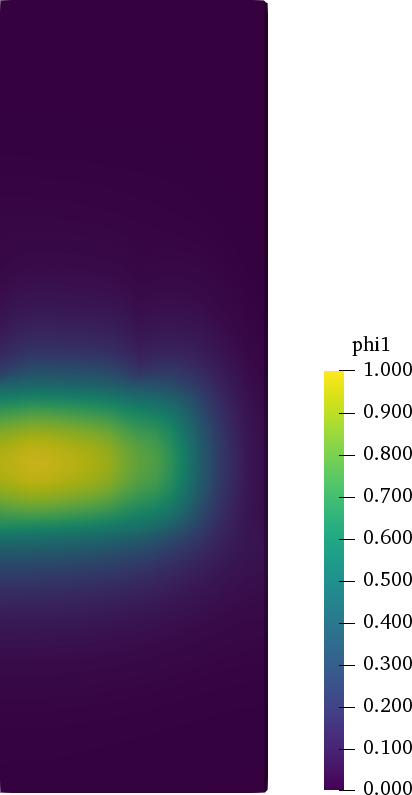
\includegraphics[width=0.25\textwidth]{abr_phi_nod_group1}}
    \hspace{0.2in}
    \subfloat[$\phi_{2}$]{
      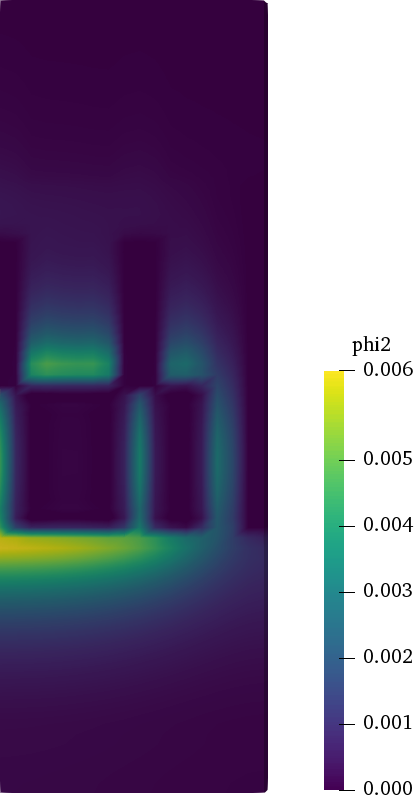
\includegraphics[width=0.25\textwidth]{abr_phi_nod_group2}}
    \caption{Fast (left) and Thermal (right) Neutron Flux in ABR.}
    \label{fig:abr_fluxes}
  \end{figure}

\section{Reactivity Coefficients}
\label{sec:reactivity_coefficients}
  Reactivity of a reactor can be used to compare the state of the reactor to the
  critical state. Reactivity $\rho$ is defined
  \begin{equation}
    \label{eq:reactivity}
    \rho \units{pcm} = \frac{\keff-1}{\keff} \times 10^5
  \end{equation}
  where \units{pcm} are units of percent-mille.
  Recall $\keff < 1$ for a subcritical reactor, $\keff=1$ for a critical
  reactor, and $\keff > 1$ for a supercritical reactor. Therefore $\rho < 0$
  for a subcritical reactor, $\rho = 0$ for a critical reactor, and $\rho > 0$
  for a supercritical reactor. 

  A reactivity coefficient can be defined as a partial derivative with respect
  to a quantity of interest \cite{textbookknief}. Let $\alpha_x$ be the 
  reactivity coefficient for quantity $x$, then
  \begin{equation}
    \label{eq:reactivity_coefficient}
    \alpha_x(x_i) = \left. \frac{\partial \rho}{\partial x} \right|_{x=x_i}
  \end{equation}
  where $\rho$ is the reactivity defined by \eref{eq:reactivity}.
  \eref{eq:reactivity_coefficient} is useful for estimating reactor dynamics.
  For some change in reactor state $\Delta x$, the reactivity response can be
  estimated as 
  \begin{equation}
    \label{eq:reactivity_estimate}
    \Delta \rho \approx \alpha_x(x_i) \, \Delta x.
  \end{equation}
  It is expected that reactivity coefficients will vary as reactor conditions
  vary. Therefore, it will be necessary to calculate $\alpha_x$ as a function of
  reactor condition $x_i$. Specifically, reactor power, $Q_{Rx}$, will be varied 
  in the calculation of $\alpha$. Therefore, consider a set of reactor powers
  varying from $0\%$ to $100\%$ as $Q_{Rx,i} = \{0\%,\ldots,100\%\}$.

  Reactivity coefficients useful for fast reactor applications include the power 
  coefficient, thermal expansion coefficient, fuel temperature (Doppler)
  coefficient, and coolant temperature coefficient (CTC) \cite{textbookknief}.
  Reactivity coefficients will be estimated with a first-order, forward-Euler,
  finite-difference approximation such that
  \begin{equation}
    \label{eq:reactivity_coefficient_finite_difference}
    \alpha_x(x_i) \approx \frac{\rho(x_i) - \rho(x_i + \Delta x)}{\Delta x}
  \end{equation}
  for a given $\Delta x$. The evaluation of
  \eref{eq:reactivity_coefficient_finite_difference} is discussed in the
  following sections for relevant reactivity coefficients.

  \subsection{Power Reactivity Coefficient}
  \label{sec:power_reactivity_coefficient}
    The power reactivity coefficient measures the reactivity response due to a 
    power increase. In a stable reactor, $\alpha_{power} < 0$ to ensure an 
    increase in reactor power requires a reactivity increase and to prevent a 
    runaway power increase. To evaluate $\alpha_{power}$, the reactor is
    simulated at a nominal reactor power, $Q_{Rx,i}$ resulting in
    $\keff(Q_{Rx,i})$. Then, reactor power is increased by $\Delta Q_{Rx}$
    resulting in $\keff(Q_{Rx,i} + \Delta Q_{Rx})$. These \keff values 
    correspond to reactivities $\rho(Q_{Rx,i})$ and 
    ${\rho(Q_{Rx,i} + \Delta Q_{Rx})}$ respectively as defined by 
    \eref{eq:reactivity}. With these values, the power reactivity coefficient 
    can be calculate as
    \begin{equation}
      \label{eq:power_reactivity_coefficient}
      \alpha_{power}(Q_{Rx,i}) = \frac{\rho(Q_{Rx,i}) - \rho(Q_{Rx,i} + 
        \Delta Q_{Rx})} {\Delta Q_{Rx}}.
    \end{equation}
    A typical value of $\Delta Q_{Rx}$ is $10\% \cdot Q_{Rx,i}$.
    % $10\% \, Q_{Rx,i}$.

  \subsection{Thermal Expansion Reactivity Coefficient}
  \label{sec:thermal_expansion_reactivity_coefficent}
    The thermal expansion reactivity coefficient describes the reactivity 
    response due solely to thermal expansion for a given increase in reactor 
    power. It is expected that thermal expansion will be the dominant 
    contribution to the power reactivity coefficient in fast reactors. This is 
    due to two main reasons: metal fuels expand significantly at high 
    temperature (see \chref{ch:thermalExpansion}) and the large neutron leakage 
    fraction (\leakage) in fast reactors \cite{PlentifulEnergy}. The leakage 
    fraction is the fraction of neutrons created in the fuel due to fission that 
    exit the core. Light Water Reactors (LWRs) typically have low and ultra-low 
    leakage designs with $\leakage \approx 2 \%$ \cite{textbookknief}. However,
    fast reactors simulated in this work have $\leakage \approx 20\%$ and 
    therefore are therefore highly sensitive to decreases in fuel density and 
    changing reactor dimensions due to thermal expansion.

    Thermal expansion temperatures, \texpfuel and \texpstruct, as implemented in 
    \chref{ch:thermalExpansion} must be known before the simulation. Note from
    \sref{sec:power_reactivity_coefficient}, a case must be simulated to
    calculate $\keff(Q_{Rx_i} + \Delta Q_{Rx})$ in the calculation of the power
    reactivity coefficient $\alpha_{power}$ in 
    \eref{eq:power_reactivity_coefficient}.  Therefore, the temperature
    distribution resulting from this study can be used to calculate the thermal
    expansion temperatures for the case with increased power, 
    ${\texp(Q_{Rx,i} + \Delta Q_{Rx})}$.
    Then, the thermal expansion reactivity coefficient is 
    \begin{equation}
      \label{eq:thermal_expansion_reactivity_coefficient}
      \alpha_{thexp}(Q_{Rx,i}) = \frac{\rho(\texp(Q_{Rx,i})) - 
        \rho(\texp(Q_{Rx,i} + \Delta Q_{Rx}))}
        {\Delta Q_{Rx}}
    \end{equation}
    where $\texp(Q_{Rx,i})$ represents the thermal expansion temperatures for
    power $Q_{Rx,i}$ and $\texp(Q_{Rx,i} + \Delta Q_{Rx})$ represents the
    thermal expansion temperatures for power $Q_{Rx,i} + \Delta Q_{Rx}$. Note
    that in \eref{eq:thermal_expansion_reactivity_coefficient}, only thermal
    expansion temperatures are changed, not the true reactor power $Q_{Rx}$.
    A typical value of $\Delta Q_{Rx}$ is $10\% \cdot Q_{Rx,i}$.
    %$10\% \, Q_{Rx,i}$.

  \subsection{Fuel Temperature (Doppler) Reactivity Coefficient}
  \label{sec:fuel_temperature_reactivity_coefficient}
    The fuel temperature reactivity coefficient measures the reactivity change 
    due to an increase in fuel temperature. This coefficient is often termed the
    Doppler coefficient because the reactivity effect is due to the Doppler
    broadening of resonance absorption peaks in heavy nuclei such as
    \isotope[238]{U} \cite{textbookknief}. Briefly, at high fuel temperatures, 
    neutrons are more likely to be parasitically absorbed by non-fissile nuclei
    than fissile-nuclei in the fuel material.

    To calculate $\alpha_{Doppler}$, fuel temperature is increased directly. A
    simulation is conducted with feedback for reactor power $Q_{Rx,i}$ and the
    temperature profile is stored. Then, the fuel temperature is uniformly 
    increased in the reactor by $\Delta T_{fuel}$ and the simulation is
    conducted again. This procedure will result in $\keff(Q_{Rx,i})$ and
    ${\keff(T_{fuel} + \Delta T_{fuel})}$. Associated reactivities can be
    calculated from \eref{eq:reactivity} and the Doppler reactivity coefficient
    follows.
    \begin{equation}
      \label{eq:doppler_reactivity_coefficient}
      \alpha_{Doppler}(Q_{Rx,i}) = \frac{\rho(Q_{Rx,i}) - \rho_i(T_{fuel} +
        \Delta T_{fuel})} {\Delta T_{fuel}}
    \end{equation}
    Note that the Doppler reactivity coefficient is always negative.
    A typical value of $\Delta T_{fuel}$ is $20\units{K}$.
    The definition in \eref{eq:doppler_reactivity_coefficient} is a
    \textit{uniform} Doppler coefficient as opposed to a \textit{distributed} 
    Doppler coefficient as temperatures are increased uniformly throughout the
    reactor.

  \subsection{\gls{ctc}}
  \label{sec:coolant_temperature_reactivity_coefficient}
    The \acrfull{ctc} describes the
    reactivity change due to an increase in coolant temperature. In \glspl{lwr}, 
    this may be called the \gls{mtc} but in fast
    reactors, the coolant is not designed to moderate neutrons. Feedback in the 
    coolant is due to two main phenomena: the decrease in absorption 
    cross-sections in the coolant due to Doppler broadening and the decrease of 
    density due to temperature increase. The dominant effect is the decrease of 
    sodium density due to the temperature increase \cite{textbookknief}.

    Unlike all other reactivity coefficients presented here, the \gls{ctc} of the 
    \gls{abr} is positive as is common in fast reactors. This implies increases 
    in coolant temperature will lead to an increase in reactivity and cause a 
    subsequent increase in reactor power. In fast reactors, the coolant acts as 
    a parasitic neutron absorber. Therefore, a decrease in the sodium absorption 
    cross-section encourages neutron absorption in fissile material in the fuel 
    resulting in a reactivity increase. This does not pose a stability problem 
    as long as the power reactivity coefficient remains negative.

    To calculate $\alpha_{CTC}$, coolant temperature is increased directly with
    a procedure similar to that for the Doppler reactivity coefficient in
    \sref{sec:fuel_temperature_reactivity_coefficient}. A simulation is 
    conducted with feedback for reactor power $Q_{Rx,i}$ and the temperature 
    profile is stored. Then, the coolant temperature is uniformly
    increased by $\Delta T_{cool}$ and the simulation is conducted again. This
    procedure will result in $\keff(Q_{Rx,i})$ and 
    ${\keff(T_{cool} + \Delta T_{cool})}$. The reactivity associated with each
    \keff can be calculated given \eref{eq:reactivity} and the coolant
    temperature coefficient is
    \begin{equation}
      \label{eq:coolant_temperature_reactivity_coefficient}
      \alpha_{CTC}(Q_{Rx,i}) = \frac{\rho(Q_{Rx,i}) - \rho(T_{cool} + 
        \Delta T_{cool})} {\Delta T_{cool}}.
    \end{equation}
    A typical value for $\Delta T_{cool}$ is $50 \units{K}$.

\section{Results}
\label{sec:results}
  Returning to the \gls{abr} MET-1000 benchmark, reactivity coefficients are 
  modeled for this reactor. The methodology and formulae from
  \sref{sec:reactivity_coefficients} are used. The reactor \keff as a function
  of reactor power is plotted in \fref{fig:keff_effects}. Note \keff decreases
  as power increases and the \keff for the case with increased sodium
  temperature is higher than all other \keff.
  
  The coefficients themselves are plotted in 
  \fref{fig:abr_reactivity_coefficients}. The combined power reactivity
  coefficient is plotted in \fref{fig:power_reactivity_coefficient}. Note,
  $\alpha_{power} < 0$ for all powers. At low reactor power, the reactivity
  coefficient is dominated by the Doppler reactivity coefficient plotted in
  \fref{fig:doppler_reactivity_coefficient}. At moderate reactor powers,
  $\alpha_{power}$ becomes less negative due to the coolant temperature
  coefficient plotted in \fref{fig:coolant_temperature_reactivity_coefficient}.
  At high reactor powers, $\alpha_{power}$ becomes more negative due to the
  dominance of the thermal expansion reactivity coefficient plotted in
  \fref{fig:thermal_expansion_reactivity_coefficient}. Should reactor power
  continue to increase beyond $100\%$ nominal value, the power reactivity
  coefficient would continue to become more negative as thermal expansion will
  continue to dominate.

  \begin{figure}
    \centering
    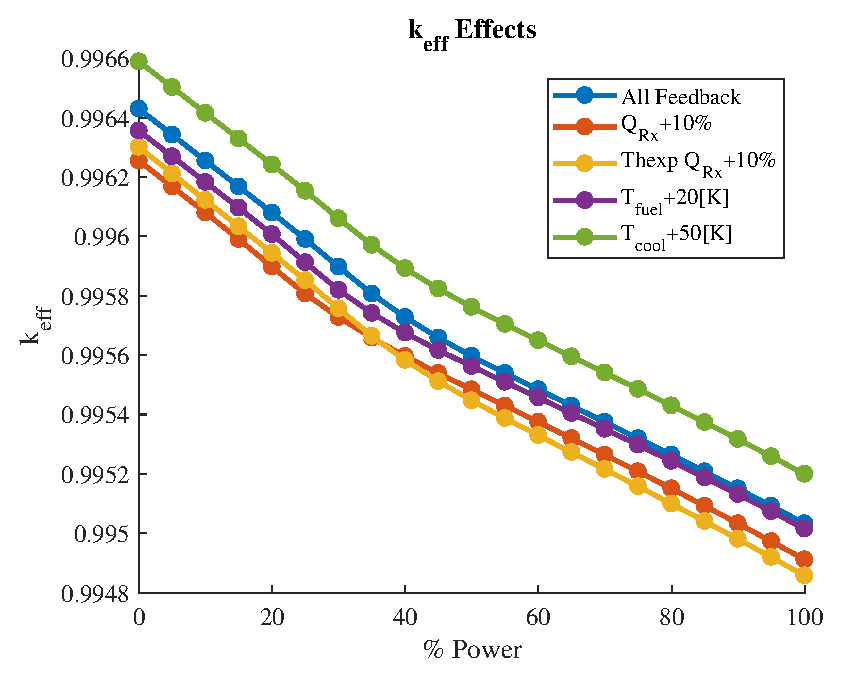
\includegraphics[width=0.7\textwidth]{keff_effects}
    \caption{Feedback Effects on \keff.}
    \label{fig:keff_effects}
  \end{figure}

  \begin{figure}
    \centering
    \subfloat[Power Reactivity Coefficient.]{
      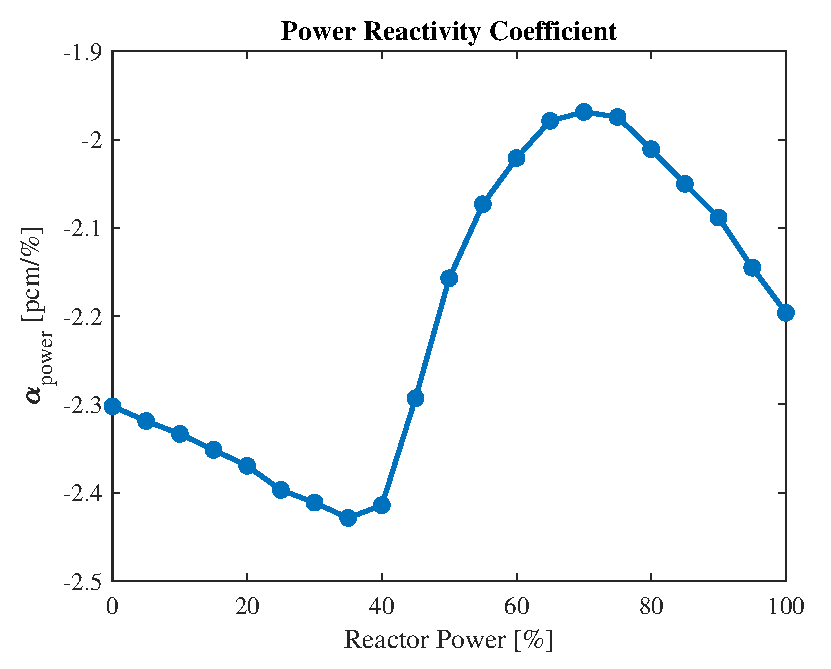
\includegraphics[width=0.5\textwidth]{alpha_power}
      \label{fig:power_reactivity_coefficient}}
    \hspace*{\fill}
    \subfloat[Thermal Expansion Reactivity Coefficient.]{
      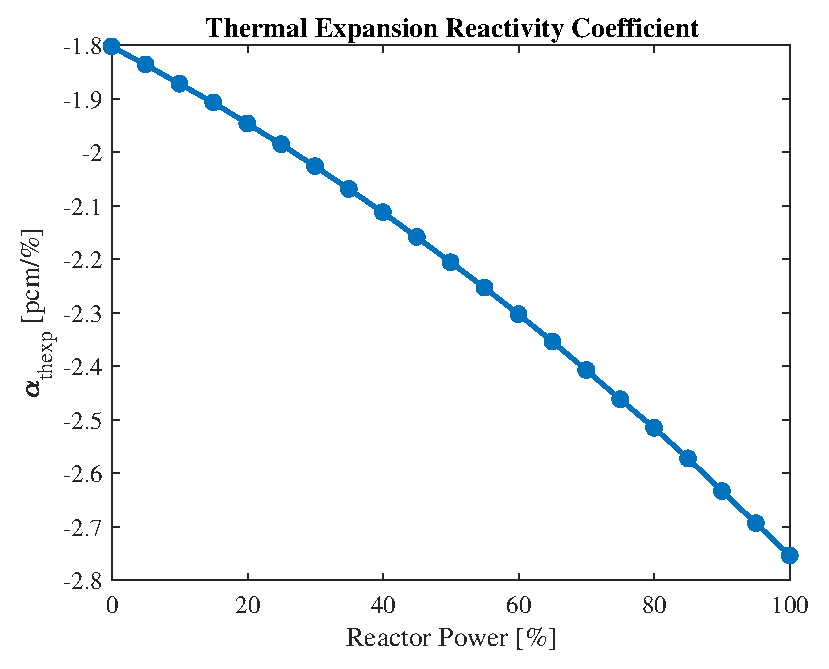
\includegraphics[width=0.5\textwidth]{alpha_thexp}
      \label{fig:thermal_expansion_reactivity_coefficient}}
    \vspace{\baselineskip}
    \subfloat[Doppler Reactivity Coefficient.]{
      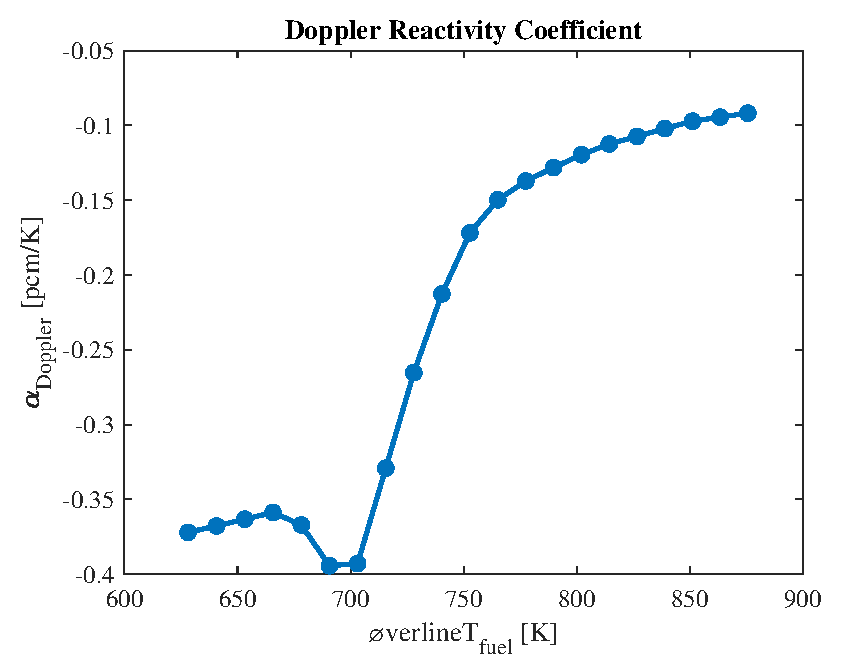
\includegraphics[width=0.5\textwidth]{alpha_fuel}
      \label{fig:doppler_reactivity_coefficient}}
    \hspace*{\fill}
    \subfloat[Coolant Temperature Reactivity Coefficient.]{
      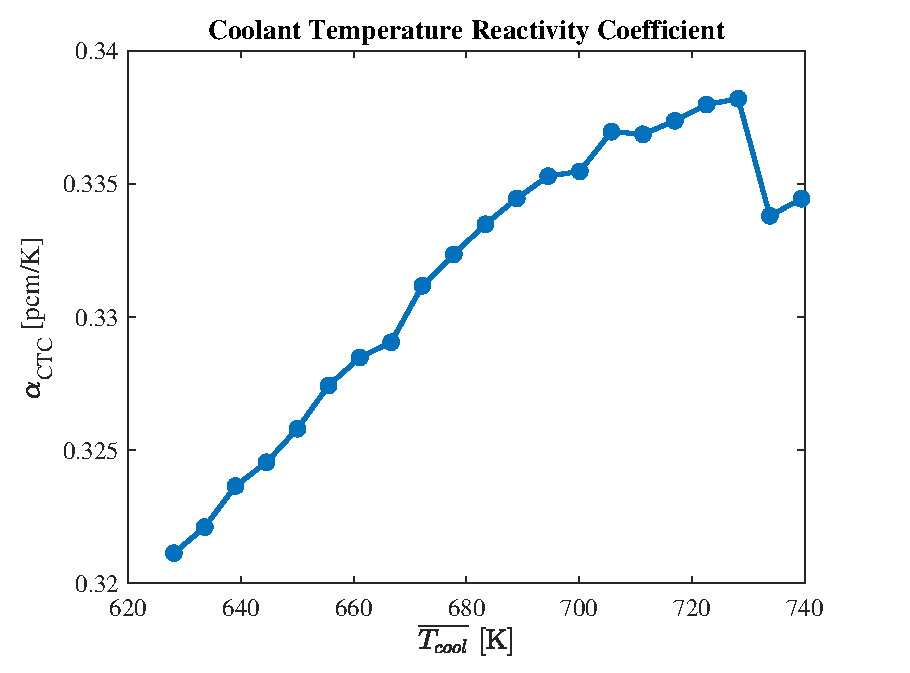
\includegraphics[width=0.5\textwidth]{alpha_cool}
      \label{fig:coolant_temperature_reactivity_coefficient}}
    \caption{ABR Reactivity Coefficients.}
    \label{fig:abr_reactivity_coefficients}
  \end{figure}
